%%%%%%%%%%%%%%%%%%%%%%%%%%%%%%%%%%%%%%%%%%%%%%%%%%%%%%%%%%%%%%%%%%%%%
%
%  This is a sample LaTeX input file for your contribution to 
%  the MC2013 conference. Modified by R.C. Martineau at INL from A. 
%  Sood at LANL, from J. Wagner ORNL who obtained the original class 
%  file by Jim Warsa, LANL, 16 July 2002}
%
%  Please use it as a template for your full paper 
%    Accompanying/related file(s) include: 
%       1. Document class/format file: mc2013.cls
%       2. Sample Postscript Figure:   figure.eps
%       3. A PDF file showing the desired appearance: template.pdf 
%    Direct questions about these files to: richard.martinea@inl.gov
%
%    Notes: 
%      (1) You can use the "dvips" utility to convert .dvi 
%          files to PostScript.  Then, use either Acrobat 
%          Distiller or "ps2pdf" to convert to PDF format. 
%      (2) Different versions of LaTeX have been observed to 
%          shift the page down, causing improper margins.
%          If this occurs, adjust the "topmargin" value in the
%          mc2013.cls file to achieve the proper margins. 
%
%%%%%%%%%%%%%%%%%%%%%%%%%%%%%%%%%%%%%%%%%%%%%%%%%%%%%%%%%%%%%%%%%%%%%


%%%%%%%%%%%%%%%%%%%%%%%%%%%%%%%%%%%%%%%%%%%%%%%%%%%%%%%%%%%%%%%%%%%%%
\documentclass{mc2013}
%
%  various packages that you may wish to activate for usage 
\usepackage{graphicx}
\usepackage{tabls}
\usepackage{afterpage}
\usepackage{cites}
\usepackage{amsmath}
\usepackage{amssymb}
%\usepackage{epsf}
%
%
% Insert authors' names and short version of title in lines below
%
\newcommand{\authorHead}      % Author's names here
   {A.Alfonsi, C. Rabiti, D. Mandelli, J.J. Cogliati, R.A. Kinoshita}  
\newcommand{\shortTitle}      % Short title here
   {Short version of title as entered by author on web page}  
%%%%%%%%%%%%%%%%%%%%%%%%%%%%%%%%%%%%%%%%%%%%%%%%%%%%%%%%%%%%%%%%%%%%%
%
%   BEGIN DOCUMENT
%
%%%%%%%%%%%%%%%%%%%%%%%%%%%%%%%%%%%%%%%%%%%%%%%%%%%%%%%%%%%%%%%%%%%%%
\begin{document}

%
%      Headers and Footers
\afterpage{%
\fancyhf{}%
\fancyhead[CE]{              
{\scriptsize \authorHead}}                                                
\fancyhead[CO]{               
{\scriptsize \shortTitle}}                  
%\lfoot{\scriptsize{
%International Conference on Mathematics and Computational Methods
%Applied to Nuclear Science \& Engineering (M\&C 2013), 
%\\ Sun Valley, Idaho, USA, May 5-9, 2013.}}%
\rfoot{\thepage/\totalpages{}}%

\pagestyle{fancy}
%\setlength{\topmargin}{-20pt}
}
 
\normalsize

%\setlength{\baselineskip}{16.8pt}
\vspace{-3pt}

% 
% TITLE
%

\begin{center}
\textbf{\large \\%
TITLE OF THE PAPER 
}
% 
% FIRST AUTHORS 
%
\\
\setlength{\baselineskip}{14pt}
\textbf{A. Alfonsi, C. Rabiti, D. Mandelli, J.J. Cogliati, R.A. Kinoshita} \\ %\footnote{Footnote, if necessary, in Times New Roman font and font size 9} 
Idaho National Laboratory  \\
2525 Fremont Avenue, Idaho Falls, ID 83415 \\
Andrea.Alfonsi@inl.gov; Cristian.Rabiti@inl.gov \\

\end{center}

%
% SET RAGGED RIGHT MARGIN
%
\raggedright


\section*{ABSTRACT} 
\begin{quote}
\begin{small}
To be added

\emph{Key Words}: Reactor Simulation, Probabilistic Risk Assessment, Dynamic PRA, Monte-Carlo, Relap-7 %, Three Miles Island, 
\end{small} 
\end{quote}

\setlength{\baselineskip}{14pt}
\normalsize

\Section{INTRODUCTION} 
RAVEN (\textbf{R} eactor \textbf{A}nalysis and \textbf{V}irtual control \textbf{EN}viroment) is a complex software tool that acts as the control logic driver for RELAP-7. The goal of this paper is to highlight the software structure of the code and its utilization in conjunction with the newly developed Thermo-Hydraylic code RELAP-7. RAVEN is a software framework that allows dispatching the following functionalities:

\begin{itemize}
\item Derive and actuate the control logic required to:
\begin{itemize}
\item Simulate the plant control system;
\item Simulate the operator actions (guided procedures);
\item Perform Monte-Carlo sampling of random distributed events;
\item Perform event tree based analysis.
\end{itemize}

\item Provide a Graphical User Interface (GUI) to:
\begin{itemize}
\item Input a plant description to RELAP-7(components, controlled variables, controlled
parameters);
\item Concurrent monitoring of Controlled Parameters;
\item Concurrent alteration of Controlled Parameters.
\end{itemize}

\item Provide a post-processing data mining capability based on:
\begin{itemize}
\item Dimensionality reduction;
\item Cardinality reduction.
\end{itemize}

\end{itemize}

The paper is divided in three main sections:
\begin{itemize}
\item RAVEN mathematical framework;
\item RAVEN software structure;
\item Demonstration of a Station Black Out (SBO) analysis of a Pressurized Water Reactor (PWR).
\end{itemize}


\Section{MATHEMATICAL FRAMEWORK}
\label{sec:mathFramework}
In the following paragraphs the mathematical framework is briefly described, analyzing the set of the
equations needed to model the control system in a nuclear power plant.

\Subsection{Plant and Control System Model} 
\label{sec:PlantControlModel}
The first step will be the derivation of the mathematical model representing, at a high level of abstraction,
the plant and control system model. Let be $\bar{\theta}(t)$ a vector describing the plant status in the phase space, and the governing equation:

\begin{equation}
\frac{\partial \bar{\theta}}{\partial t} = \bar{H}(\theta(t),t)
\label{eq:SystemDynamics}
\end{equation}

In the above equation we have assumed the time differentiability in the phase space. This is in generally
not required and it is abused here for compactness of the notation. Now an arbitrary decomposition of the
phase space is performed:

\begin{equation}
\bar{\theta}=\binom{\bar{x}}{\bar{v}}
\label{eq:firstDecomposition}
\end{equation}

The decomposition is made in such a way that $x$ represent the unknowns solved by RELAP-7, while $v$ are the variables directly controlled by the control system . The governing equation is now casted in a system of equations:

\begin{equation}
\begin{cases} 
\frac{\partial \bar{x}}{\partial t} = \bar{F}(\bar{x},\bar{v},t) \\ 
\frac{\partial \bar{v}}{\partial t} = \bar{V}(\bar{x},\bar{v},t) \\
\end{cases}
\label{eq:generalSystemEquation}
\end{equation}

As a consequence of this splitting, the contains components state variables of the phase space now that
are continuous while contains all variables describing the discrete state variables that are of the system
usually handled by the control system. As a next step, we realize that the function 
$\bar{V}(\bar{x},\bar{v},t)$ 
representing the control system, does not depend on the knowledge of the complete status of the system but on a restricted subset that we call control variables $\bar{C}$:

\begin{equation}
\begin{cases} 
\frac{\partial \bar{x}}{\partial t} = \bar{F}(\bar{x},\bar{v},t) \\
\bar{C} = \bar{G}(\bar{x},t) \\ 
\frac{\partial \bar{v}}{\partial t} = \bar{V}(\bar{x},\bar{v},t) 
\end{cases}
\label{eq:generalSystemEquationwithControl}
\end{equation}

where 
$\bar{C}$
is a vector which having lesser dimensionality than
$\bar{x}$
and therefore is more convenient to work with. In rest of this document the following naming will be adopted: $\bar{C}$: monitored variables $\bar{v}$:
controlled variables.
Note that even if it seems more appropriate, the standard naming of signals (monitored)
and status (controlled) is not yet used. The reason for this choice is that, the chosen naming better mirrors
the computational pattern between RAVEN and RELAP 7 and moreover the definition of signals is more
tight to the definition of the control logic for each component and therefore relative rather than absolute in
the overall system analysis. In fact we could have signal for a component that are status of another creating
a definition that would be not unique. Another reason is that the standard naming will loose every meaning
once used also for uncertainty analysis.

\Subsection{Operator Splitting Approach} 
\label{sec:operatorSplitting}

System of equations shown in Eq.~\ref{eq:generalSystemEquationwithControl} is, generally speaking, fully coupled and in the past it has always been solved following an operator splitting approach. The reasons for this choice are several:

\begin{itemize}
\item Control system reacts with an intrinsic delay anyhow;
\item The reaction of the control system might move the system between two different discrete state and
therefore numerical errors will be always of first order unless the discontinuity will be treated explicitly.
\end{itemize}

RAVEN is, thus, using this approach. Therefore Eq.~\ref{eq:generalSystemEquationwithControl} becomes:

\begin{equation}
\begin{cases} 
\frac{\partial \bar{x}}{\partial t} = \bar{F}(\bar{x},\bar{v}_{t_{i}-1},t) \\
\bar{C} = \bar{G}(\bar{x},t) \\ 
\frac{\partial \bar{v}}{\partial t} = \bar{V}(\bar{x},\bar{v}_{t_{i}-1},t) 
\end{cases}
\label{eq:generalSystemEquationwithControlSplitting}
\end{equation}
\Section{SOFTWARE STRUCTURE} 
RELAP-7 is the solver for the plant system except for the control system. From the mathematical
formulation presented so far, RELAP-7 will solve 
$\frac{\partial \bar{x}}{\partial t} = \bar{F}(\bar{x},\bar{v}_{t_{i}-1},t)$.
\begin{figure}[h] \label{fig:ControlSoftwareLayout}
  \centering
     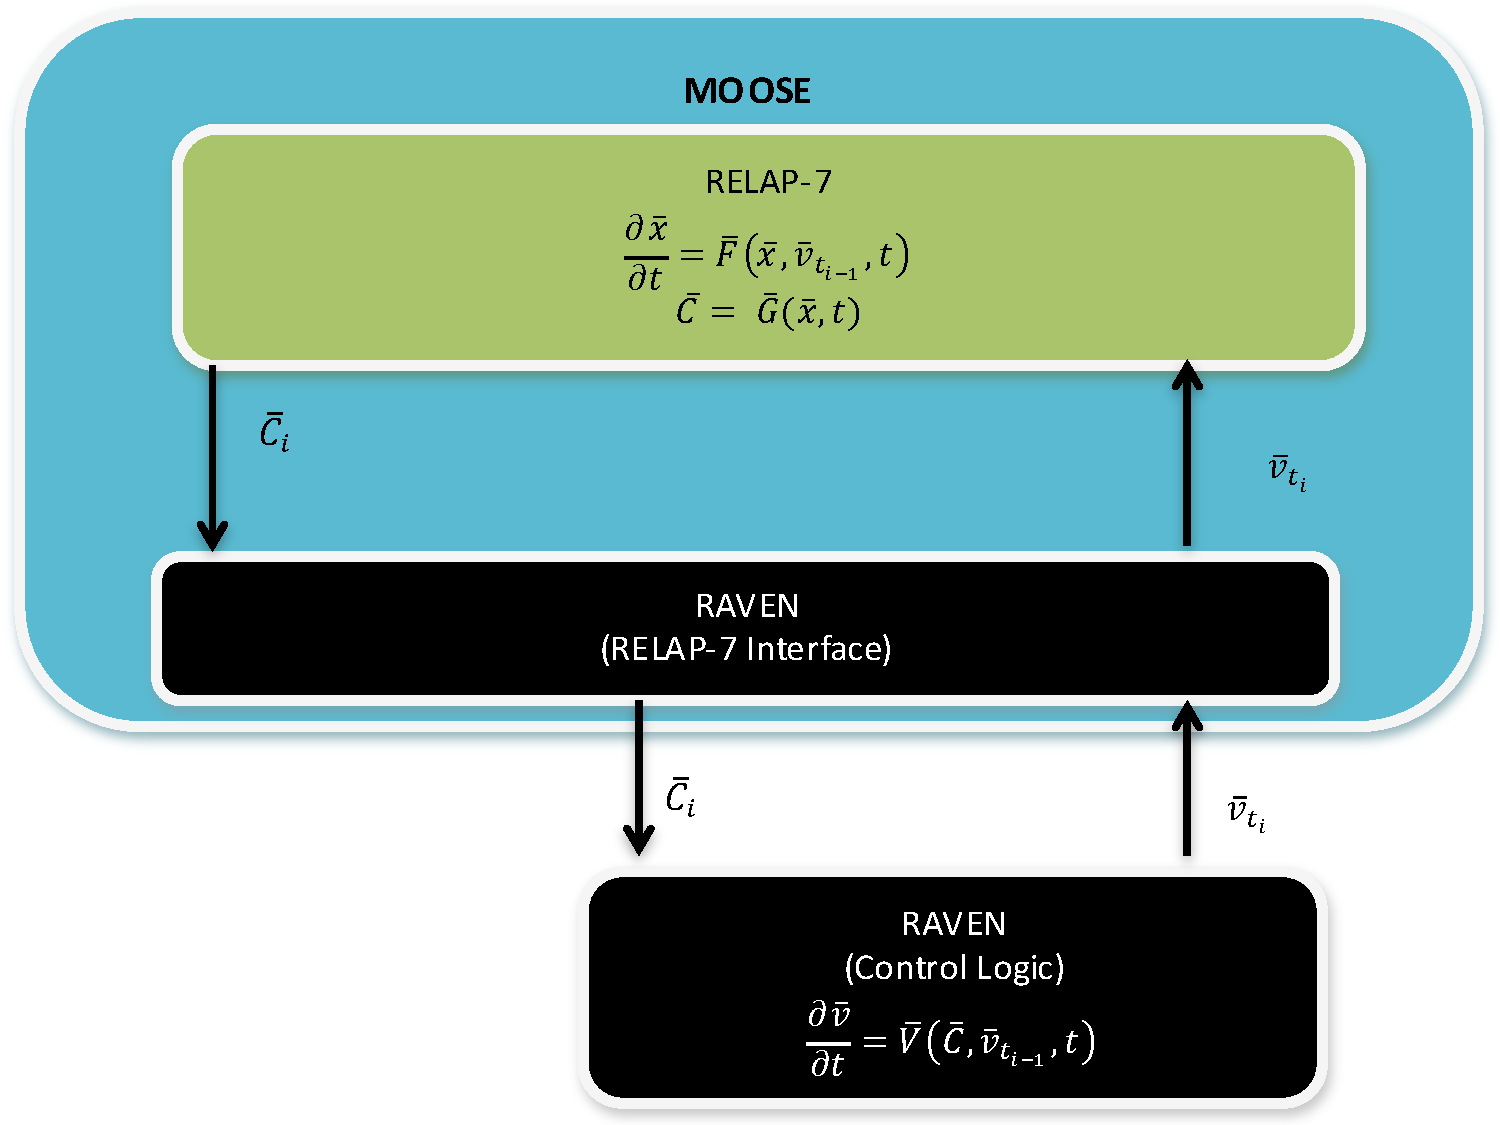
\includegraphics[width=0.5\textwidth]{figures/ControlSystemSoftwareLayout.pdf}
  \caption{Control System Software Layout.}
\end{figure}
RELAP-7 will be based on the middleware software MOOSE, that, in addition to provide the algorithms for the solution of the differential equation, will also provide all the manipulation tools for the C++ classes containing the solution vector. More in detail the plant is represented by a set of components and each component type corresponds to a C++ class.
At each time step RELAP-7/MOOSE will update the information within the classes with the current solution  $\bar{x}$, then RAVEN will ask MOOSE to perform the needed manipulation to construct the monitored quantities $\bar{C}$. Once $\bar{C}$ is constructed, the information is reduced to a vector of
numbers understandable by the control system. The equation 
$\frac{\partial \bar{v}}{\partial t} = \bar{V}(\bar{x},\bar{v}_{t_{i}-1},t) $
is solved and the set of control parameters for the next time step $v_{t_{i}}$ is obtained. 
Up to know no situations where the complexity of the equation 
$\frac{\partial \bar{v}}{\partial t} = \bar{V}(\bar{x},\bar{v}_{t_{i}-1},t) $
is solved and the set of control parameters for the next time step $v_{t_{i}}$ required a numerical solution therefore for the moment RAVEN remains numerical integration free. 
Note that once the information is transferred to $C$, the way through which the plant
solution $x$ is computed or stored is irrelevant. The last statement highlights the capability of RAVEN to
represent an easily generalizable tool. This functional scheme is represented in Figure~\ref{fig:ControlSoftwareLayout}.
To be more specific, in reality MOOSE is made aware of the need to compute at the end of each time step the $C$ as a consequence this is immediately available at the end of each time step. As a consequence scheme in Figure ?? is more accurate in terms of software implementation. In the following of the discussion depending of which aspect will be more relevant either scheme in Figure~\ref{fig:ControlSoftwareLayout} or ?? will be referred.
\begin{figure}[h] \label{fig:CalcFlow1}
  \centering
     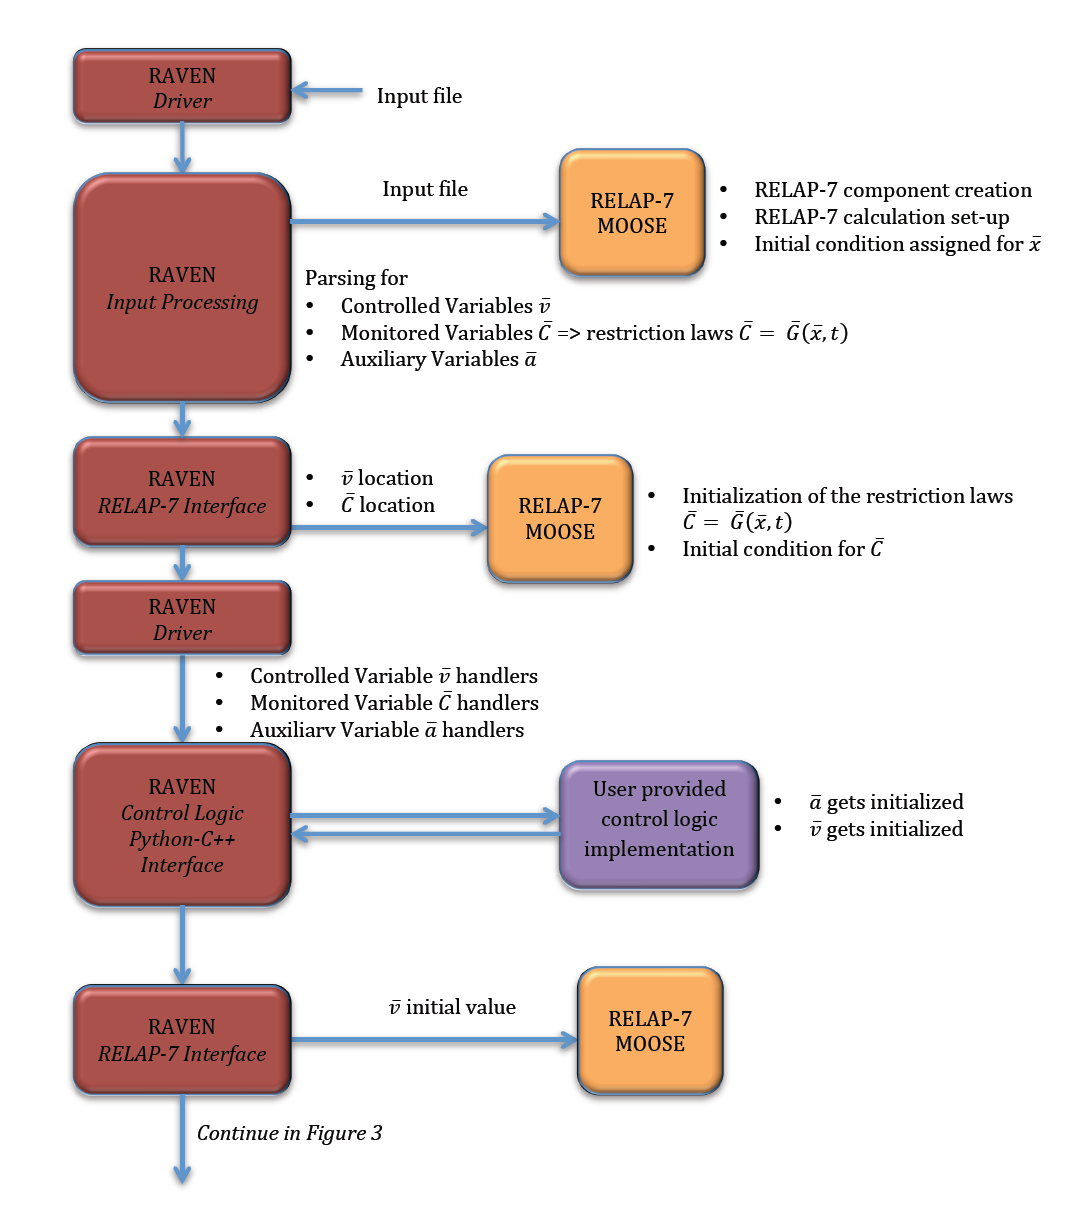
\includegraphics[width=0.8\textwidth]{figures/CalculationFlow_part_1.PNG}
  \caption{Control System Software Layout.}
\end{figure}
\begin{figure}[h] \label{fig:CalcFlow2}
  \centering
     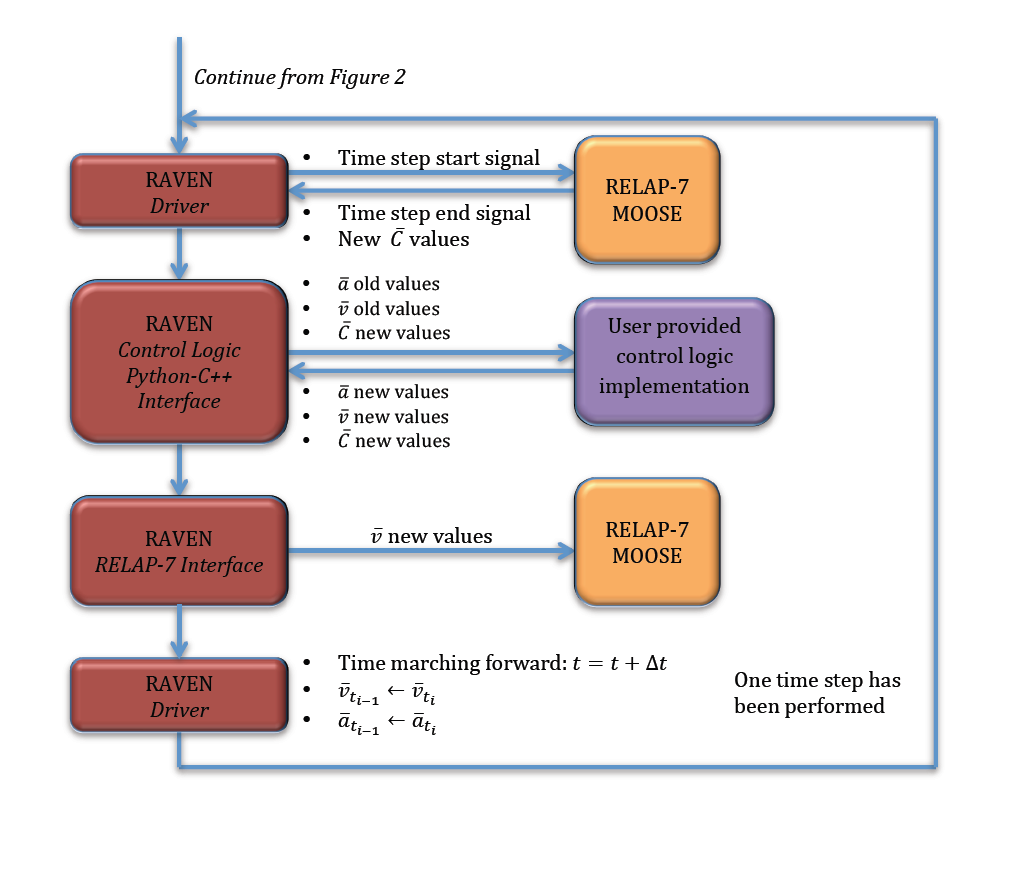
\includegraphics[width=0.8\textwidth]{figures/CalculationFlow_part_2.PNG}
  \caption{Control System Software Layout.}
\end{figure}
\Section{CONCLUSIONS}

[]


%\Section*{REFERENCES}
\setlength{\baselineskip}{12pt}
\begin{thebibliography}{300}
\bibitem{journal} B. Author(s), ``Title,'' {\it Journal Name in Italic}, 
          {\bf Volume in Bold}, pp. 34-89 (19xx).
\bibitem{proc_paper} C. D. Author(s), ``Article Title,'' {\it Proceedings of
          Meeting in Italic}, Location, Dates of Meeting, Vol. n, pp. 134-156 
          (19xx).
\bibitem{book} E. F. Author, {\it Book Title in Italic}, Publisher, City \&
          Country (19xx). 
\bibitem{website} ``Spallation Neutron Source: The next-generation 
          neutron-scattering facility in the United States,'' 
          http://www.sns.gov/documentation/sns\_brochure.pdf (2002).
\end{thebibliography}

\end{document}


